\chapter{Methodology}\label{ch:methodology}
\epigraph{\textit{\normalsize “Artificial intelligence, in fact, is obviously an intelligence transmitted by conscious subjects, an intelligence placed in equipment.”}}{\textit{ \normalsize Pope Benedict XVI}}

The first step would be to implement the state-of-the-art in image regeneration to guage the improvements. We use DCGAN to start of with. The results of the training and testing will be recorded to compare it with the results of our CapsNet-based approach later. We will be using CapsNet as the underlying technology to implement our GAN (CapsGAN). The goal is to replace the CNN inside DCGAN with CapsNet and compare the results. The GAN internally consists of two components - a generator and a discriminator - which we build out of CapsNet. The discriminator is initially trained separately to distinguish real and fake data, and later they work together to improve upon their performance by acting as adversaries.
\par\bigskip

\begin{figure}[H]
\centering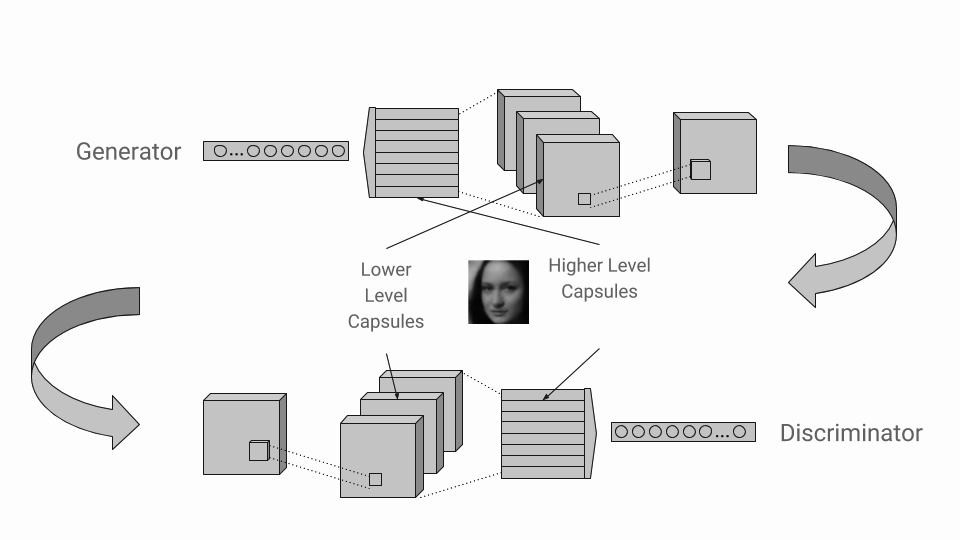
\includegraphics[width=1\textwidth]{images/methodology.png}
\caption{Proposed architecture}
\end{figure}

The generator will use noise as input to generate faces. We will use random data as this noise. This ensures the data is unique and across the spectrum while retaining a normal distribution.
\par\bigskip

The CapsNet making up the discriminator consists of a small convolutional network to convert low level data in the form of pixels into an artifact called "pose". These poses can be anything, like nose, ear, eye, etc. These poses are then passed on as input to the later lower layers consisting of components called Capsules. A capsule is analogous to the human brain containing different modules to handle different tasks. The brain has a mechanism to route the information among the modules, to reach the best modules that can handle the information.
\par\bigskip

A capsule is a nested set of neural layers. Each capsule is able to handle one particular pose and communicate its calculation to other capsules which can use that calculation. This calculation is in the form of a probability prediction of the current pose that takes place in its logistic unit. This working is fundamentally different from convolutional networks, which utilizes Max Pooling. Max pooling selects the most active input node from the next layer to pass on the information. CapsNet on the other hand selects the next capsule based on which capsule would be capable of handling that information. This is called Dynamic routing. This results in invariance of information to the position and orientation of features in an object while ignoring the invariance in very low level features as, at the pixel level, this does not matter.
\par\bigskip

The generator is built using an architecture that is a mirror image of the discriminator. Inside, the data flow is in the opposite direction. The job of the discriminator is to take the images given out by the generator and discriminate it against a ground truth. The discriminator selects the class based on how close the images are in agreement. The underlying principle is that when multiple entities agree with each other in higher dimensions, the chances of it happening due to complete coincidence is exponentially minimal. This ensures the understanding by the CapsNet of the world is remarkably similar to humans.